\begin{figure*}
  \centering
  \begin{subfigure}[b]{\textwidth}
    \centering
    % \begin{noindent}
    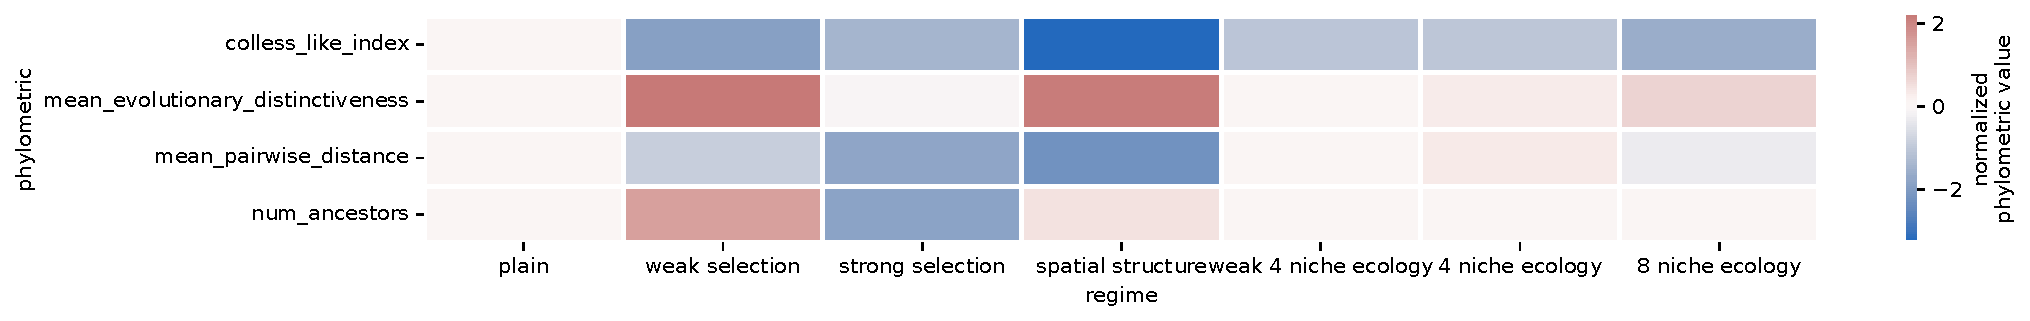
\includegraphics[width=\textwidth]{binder/binder/teeplots/epoch=0+mut_distn=np.random.standard_normal+viz=heatmap+x=regime+y=phylometric+ext=.pdf}
    \caption{%
      gaussian mutation distribution at epoch 0 (generation 32,768)}
    \label{fig:perfect-tree-phylometrics-heatmap-sensitivity-analysis:epoch0}
    % \end{noindent}
  \end{subfigure}
  \begin{subfigure}[b]{\textwidth}
    \centering
    % \begin{noindent}
    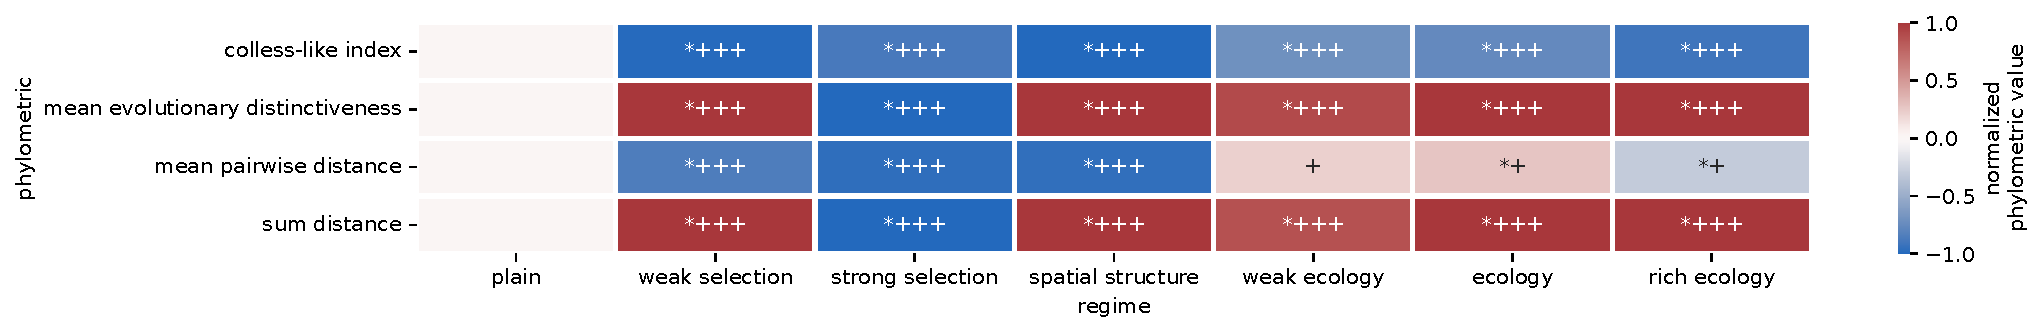
\includegraphics[width=\textwidth]{binder/binder/teeplots/epoch=2+mut_distn=np.random.standard_normal+viz=heatmap+x=regime+y=phylometric+ext=.pdf}
    \caption{%
      gaussian mutation distribution at epoch 2 (generation 98,304)}
    \label{fig:perfect-tree-phylometrics-heatmap-sensitivity-analysis:epoch2}
    % \end{noindent}
  \end{subfigure}
  \begin{subfigure}[b]{\textwidth}
    % \begin{noindent}
    \centering
    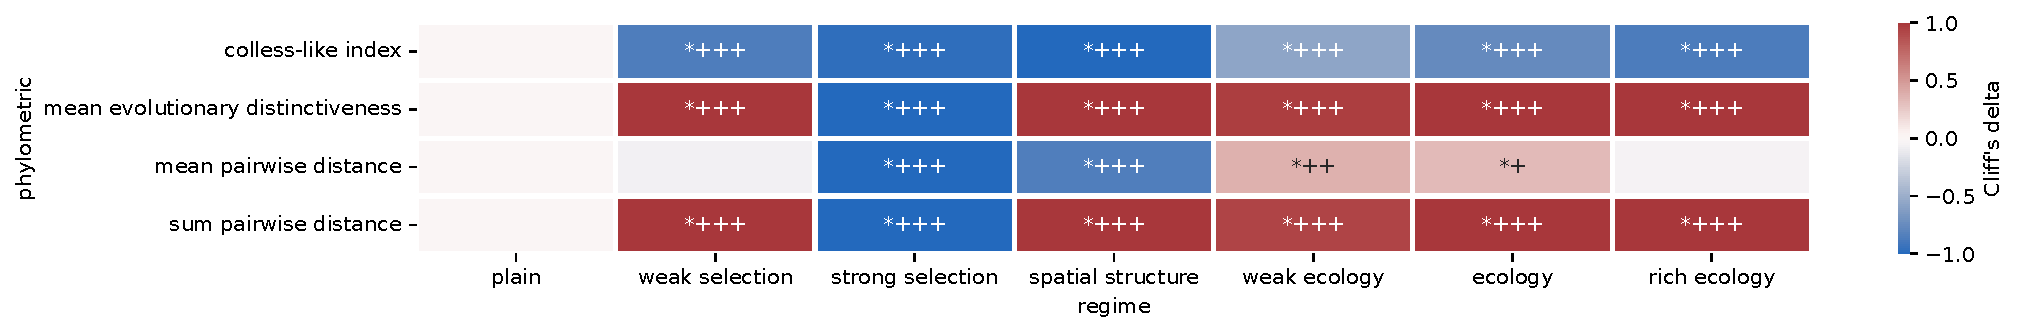
\includegraphics[width=\textwidth]{binder/binder/teeplots/epoch=7+mut_distn=np.random.exponential+viz=heatmap+x=regime+y=phylometric+ext=.pdf}
    \caption{%
      exponential mutation distribution at epoch 7 (generation 262,144)}
    \label{fig:perfect-tree-phylometrics-heatmap-sensitivity-analysis:exponential}
    % \end{noindent}
  \end{subfigure}
  \caption{%
    Sensitivity analysis results for normalized tree phylometrics across surveyed evolutionary regimes, calculated on perfect-fidelity simulation phylogenetic records.
    Normalized tree phylometrics are depicted as a heatmap for each sensitivity analysis condition.
  }
  \label{fig:perfect-tree-phylometrics-heatmap-sensitivity-analysis}
\end{figure*}
